






\documentclass[11pt]{article}
\usepackage[margin=1in]{geometry}
\usepackage{amsmath, amssymb, amsthm}
\usepackage{physics}
\usepackage{bm}
\usepackage{hyperref}
\usepackage{graphicx}
\usepackage{enumitem}
\usepackage{siunitx}
\usepackage{mathtools}
\usepackage{braket}
\usepackage{quantikz}
\usepackage{tikz}
\usepackage{tikz-3dplot}
\usetikzlibrary{arrows.meta,calc}
\usepackage{MnSymbol,wasysym}
\newenvironment{summary}{\par\noindent\textbf{Summary.} }{\par}

\title{CSCI-739 Quantum Machine Learning \\[4pt] \large Homework 3}
\date{}

\begin{document}
\maketitle

\begin{center}
\textit{You got this, team. These problems are not arbitrary—they are designed as a journey through the essential pillars of QML. You will see how phase imperfections affect quantum operations (P1), how finding and approximating ground states links quantum physics to learning (P2), how the XOR problem illustrates quantum feature mappings and circuit expressivity (P3), and how quantum kernels power classification in QSVMs, and when entanglement in them actually helps (P4). The bonus problem pushes you deeper: it connects theory to optimization behavior and barren plateaus. Each step builds intuition that scales from single-qubit reasoning to multi-qubit learning architectures. If you can reason through these, you’re already thinking like a quantum scientist. I believe in you all! \smiley{}}
\end{center}

\vspace{1em}

\noindent
*ahem, inspirational speech* \newline
Quantum machine learning is a blend of physics, computer science, and mathematics—a true frontier field. The first four problems of this homework each connect to a core competency we are developing in the course:
\begin{itemize}
  \item \emph{P1 (Phase-deformed $X$ gates):} illustrates how coherent errors and gate deformations influence measurement outcomes, tying physical noise to computational results.
  \item \emph{P2 (Ground states and VQCs):} demonstrates how energy minimization connects to learning and how variational quantum circuits approximate eigenstates.
  \item \emph{P3 (XOR and encoding strategies):} shows how quantum encodings and an entangling gate let a small circuit learn a problem that is not linearly separable, and generalize to noisy data.
  \item \emph{P4 (Quantum SVMs):} bridges classical ML concepts with quantum kernels, and tests whether entanglement in the feature map actually helps.
  \item \emph{Bonus:} expands your understanding of gradient theory and scaling, preparing you for advanced QML topics like quantum optimization and barren plateau analysis.
\end{itemize}
Use lectures, notes, the internet, and each other to research the problems and conquer this homework, team! Have fun \smiley{}! Also:

\begin{figure}[h!]
\centering
\vspace{1em}
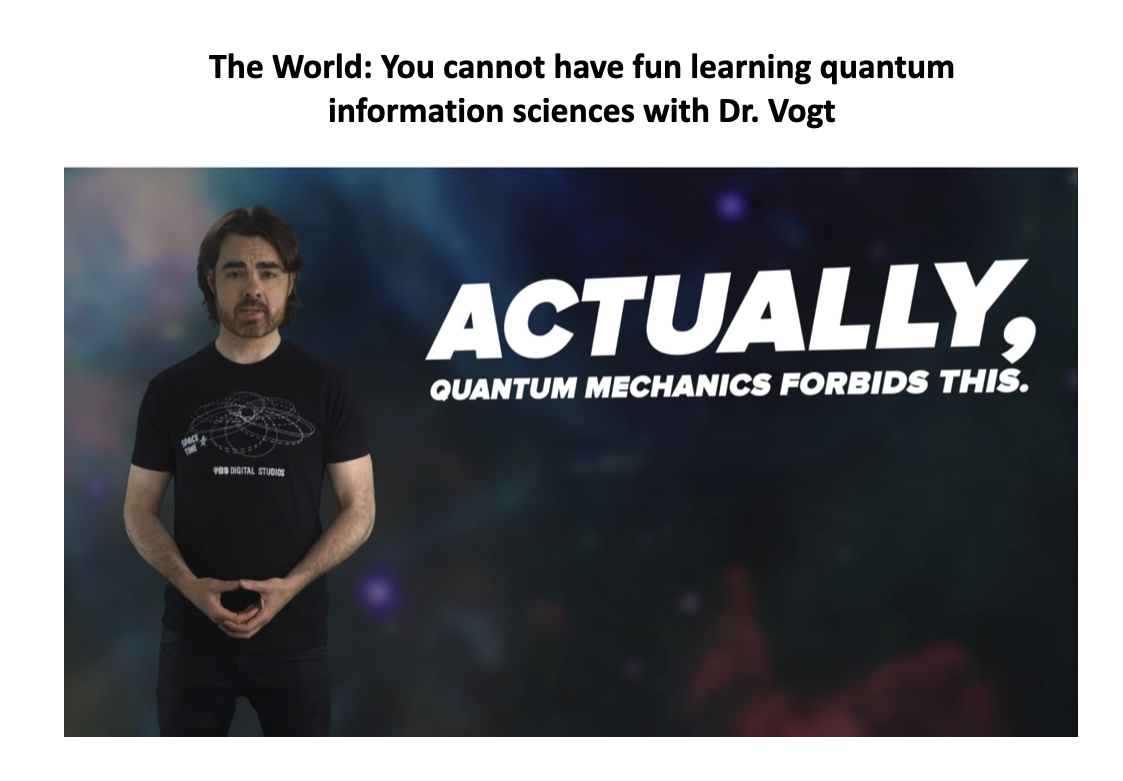
\includegraphics[width=0.75\textwidth]{quantumvogt.png}
\vspace{0.5em}
\end{figure}
% ============================================ 
\newpage
\section*{Problem 1 — A Phase-Deformed $X$ Gate and Measurement Effects (25 pts)}

\begin{summary}
We study a one-parameter family of unitaries $X(\varepsilon)$ that reduces to the Pauli-$X$ gate at $\varepsilon=0$, but deviates by a coherent (phase-induced) deformation when $\varepsilon\neq 0$. You will analyze measurement statistics for a single application ($n=1$) and for repeated applications ($n$ general), and reason about whether one can tune $\varepsilon$ to achieve arbitrary measurement probabilities compared to the ideal case.
\end{summary}

Define
\[
X(\varepsilon)\;=\;
\begin{pmatrix}
\sin\varepsilon & \cos\varepsilon\\[4pt]
\cos\varepsilon & -\sin\varepsilon
\end{pmatrix}
\;=\;
\cos\varepsilon\,X \;+\; \sin\varepsilon\,Z.
\]

\begin{enumerate}[label=(\alph*)]
\item \textbf{Check the limits and unitarity.}
Show that $X(0)=X$. Prove that $X(\varepsilon)$ is unitary (and Hermitian), and verify $X(\varepsilon)^2=I$.

\item \textbf{Special case $n=1$ from $\ket{0}$.}
Prepare $\ket{0}$ and apply $X(\varepsilon)$ once:
\[
\ket{\psi_1(\varepsilon)} \;=\; X(\varepsilon)\ket{0}
\;=\; \sin\varepsilon\,\ket{0} \;+\; \cos\varepsilon\,\ket{1}.
\]
Compute the measurement probabilities in the computational basis:
\[
P_{\varepsilon}^{(1)}(0),\qquad
P_{\varepsilon}^{(1)}(1),
\] and verify their sum is 1.
Compare the cases $\varepsilon=0$ (ideal $X$) and $\varepsilon\neq 0$. \emph{Question:} by choosing $\varepsilon$, can you achieve \emph{any} target probability $P(1)\in[0,1]$ in this single-application setting?

\item \textbf{General $n$ applications from $\ket{0}$.}
Using $X(\varepsilon)^2=I$, compute

\[
\ket{\psi_n(\varepsilon)} \;=\; X(\varepsilon)^n  \ket{0},
\] Hint: the result differs for even and odd $n$ \smiley{}.
Compute $P_{\varepsilon}^{(n)}(0),P_{\varepsilon}^{(n)}(1)$ and compare to the ideal ($\varepsilon=0$). \emph{Question:} for general $n$, can you still set $P(1)$ arbitrarily by tuning $\varepsilon$ (and therefore $P(0)$)? Discuss the parity effect.

\item Comment on why the ideal versus the error-prone unitary operation is concerning, especially if we do not know exactly what $\varepsilon$ is in practice on NISQ-era hardware. Comment on why quantum error correction is therefore so critical.  
\end{enumerate}

% ============================================
\section*{Problem 2 — Ground State Analytically, Then via a VQC (25 pts)}

\begin{summary}
This problem introduces the ground state (variational eigenvalue) problem. You will first compute the eigenvalues and eigenvectors of a simple $2\times2$ Hamiltonian analytically, then connect this to finding the minimal energy (ground state energy) and design a minimal variational quantum circuit (VQC) to reproduce that ground state through optimization.
\end{summary}

Consider the one-qubit Hamiltonian:
\[
H \;=\; \tfrac{1}{2}Z \; - \; X
\;=\;
\begin{pmatrix}
\tfrac{1}{2} & -1\\[4pt]
-1 & -\tfrac{1}{2}
\end{pmatrix}.
\]

\begin{enumerate}[label=(\alph*)]
  \item \textbf{Eigenvalues and eigenvectors.}  
  Find all eigenvalues and normalized eigenvectors of $H$. Write the eigenvectors explicitly in the computational basis $\{\ket{0},\ket{1}\}$. Confirm that the matrix is Hermitian and that the eigenvectors form an orthonormal basis.

  \item \textbf{Ground state problem.}  
  Define what is meant by the \emph{ground state} and \emph{ground state energy} of a Hamiltonian in quantum mechanics. Using your results from part (a), identify the ground state energy $E_0$ and the corresponding ground state $\ket{\psi_0}$.

  \item \textbf{Variational quantum circuit (VQC) approach.}  
Using the variational principle, propose a simple one-qubit ansatz such as
\[
\ket{\psi(\theta)} = R_y(\theta)\ket{0} = \cos\tfrac{\theta}{2}\ket{0} + \sin\tfrac{\theta}{2}\ket{1},
\]
and compute
\[
C(\theta) = E(\theta)  =  \bra{\psi(\theta)}H\ket{\psi(\theta)}.
\]
\begin{enumerate}[label=(\roman*)]
  \item \emph{Analytic minimizer.} Derive \(\theta_\star\) that minimizes \({E(\theta)}\) in closed form. Report \({\theta_\star}\) and \({E(\theta_\star)}\).
  \item \emph{Numerical VQE.} Implement a tiny VQE loop (e.g., grid search, Nelder–Mead, SPSA, or gradient descent) to minimize \({E(\theta)}\). For a general cost function $C(\boldsymbol{\theta})$
with parameters $\boldsymbol{\theta}=(\theta_1,\ldots,\theta_k)\in\mathbb{R}^k$ and gradient
\[
\nabla_{\boldsymbol{\theta}} C
=\Big(\tfrac{\partial C}{\partial\theta_1},\ldots,\tfrac{\partial C}{\partial\theta_k}\Big)^{\!\top}.
\]
Parameter-shift rule for one component:
\[
\frac{\partial C(\theta)}{\partial\theta}
=\frac{1}{2}\Big[C\!\big(\theta+\tfrac{\pi}{2}\big)-C\!\big(\theta-\tfrac{\pi}{2}\big)\Big].
\]
\textbf{Clarification:} this is \emph{one component} of $\nabla_{\boldsymbol{\theta}} C$.
For a $k$-parameter circuit,
\[
\frac{\partial C}{\partial\theta_i}
=\frac{1}{2}\Big[C(\boldsymbol{\theta}+\tfrac{\pi}{2}\mathbf{e}_i)-C(\boldsymbol{\theta}-\tfrac{\pi}{2}\mathbf{e}_i)\Big].
\]
Here, \(\mathbf{e}_i\) denotes the standard basis vector in parameter space \(\mathbb{R}^k\), i.e.,
\[
\mathbf{e}_i = (0,0,\ldots,1,\ldots,0)^{\top},
\]
with a single \(1\) in the \(i\)-th position and zeros elsewhere. It isolates the \(i\)-th parameter so that the shift applies only to \(\theta_i\) while keeping all other parameters fixed.

Report: (1) the optimized parameter \({\hat\theta}\), (2) the achieved value \({E(\hat\theta)}\), and (3) whether \({\hat\theta}\) (modulo \({2\pi}\) and global phase) matches your analytic \({\theta_\star}\).
  \item \emph{Measurement note.} Measure in the $Z$ basis for $Z$, and insert a Hadamard before measurement for $X$—this rotation transforms $X$ into $Z$ so that the same measurement hardware can capture both components accurately.
\end{enumerate}
\end{enumerate}

% ============================================
\section*{Problem 3 — The XOR Problem and Encoding Strategies with Variational Circuits (25 pts)}

\begin{summary}
This problem connects quantum data encoding to a fundamental classical learning challenge: the XOR classification problem, the smallest classification problem that is not linearly separable. Instead of only the four corner points, you will work with a \emph{noisy} XOR dataset, so that the model has to generalize to unseen points. You will compare basis and angle encodings, and test what the entangling gate in a variational quantum circuit (VQC) contributes. For this problem use, for example, $S=100$ shots, or your favorite number \smiley{}.
\end{summary}

\noindent\textbf{The XOR truth table.}
\[
\begin{array}{c|c|c}
x_1 & x_2 & \text{Output (XOR)} \\ \hline
0 & 0 & 0 \\ 0 & 1 & 1 \\ 1 & 0 & 1 \\ 1 & 1 & 0
\end{array}
\]

\noindent\textbf{Noisy XOR dataset (used in Problems 3 and 4).}
Each point is drawn by picking one of the four corners $c\in\{0,1\}^2$ uniformly at random and adding Gaussian noise, $x = c + \sigma\,\xi$ with $\xi\sim\mathcal{N}(0,I_2)$ and $\sigma=0.15$. The label is the XOR of the corner, $y = c_1 \oplus c_2$. Use $N=40$ training points and $200$ test points, generated with
\begin{verbatim}
import numpy as np
def noisy_xor(n, sigma, seed):
    rng = np.random.default_rng(seed)
    corners = np.array([[0, 0], [0, 1], [1, 0], [1, 1]])
    k = rng.integers(0, 4, n)
    X = corners[k] + sigma * rng.normal(size=(n, 2))
    y = corners[k, 0] ^ corners[k, 1]      # labels in {0, 1}
    return X, y
X_train, y_train = noisy_xor(40, 0.15, seed=1)
X_test,  y_test  = noisy_xor(200, 0.15, seed=2)
\end{verbatim}
Report training \emph{and} test accuracy for every model below, where a point is classified as $1$ when the model output exceeds $\tfrac12$.

\medskip
\noindent\textbf{Circuit conventions.} Qubit $0$ carries $x_1$ and qubit $1$ carries $x_2$. Both encodings below are followed by the same trainable layer
\[
V(\boldsymbol{\theta}) \;=\; \mathrm{CNOT}_{0\to1}\,\big(R_y(\theta_0)\otimes R_y(\theta_1)\big),
\qquad \boldsymbol{\theta}=(\theta_0,\theta_1),
\]
and the model output $f_{\text{VQC}}(x;\boldsymbol{\theta})$ is the probability of measuring $\ket{1}$ on qubit $1$ (the CNOT target).

\begin{enumerate}[label=(\alph*)]
\item \textbf{Basis encoding.}
Round each feature to a bit, $b_k = 1$ if $x_k>\tfrac12$ and $b_k=0$ otherwise, and prepare $\ket{b_1b_2}$ by applying the appropriate $X$ gates (or none) to $\ket{00}$. Apply $V(\boldsymbol{\theta})$, train $\boldsymbol{\theta}$, and report the learned parameters and the accuracies. Then remove the CNOT from $V$ and retrain. Explain why the model without the CNOT cannot learn XOR, no matter how $\boldsymbol{\theta}$ is chosen.

\item \textbf{Angle encoding.}
Encode the raw features as rotations, $\ket{\phi(x)} = \big(R_y(\pi x_1)\otimes R_y(\pi x_2)\big)\ket{00}$, and apply the same $V(\boldsymbol{\theta})$.
\begin{enumerate}[label=(\roman*)]
\item Show that, with the CNOT,
\(
\langle Z\rangle_{\text{qubit }1} = \cos(\pi x_1+\theta_0)\,\cos(\pi x_2+\theta_1),
\)
and that without it $\langle Z\rangle_{\text{qubit }1} = \cos(\pi x_2+\theta_1)$. (Hint: conjugating $I\otimes Z$ by a CNOT gives $Z\otimes Z$.)
\item Use (i) to find, by hand, a $\boldsymbol{\theta}_\star$ that classifies the four corners perfectly.
\item Train $\boldsymbol{\theta}$ on the noisy data, report the accuracies, and compare $\hat{\boldsymbol{\theta}}$ with $\boldsymbol{\theta}_\star$.
\end{enumerate}

\item \textbf{Objective function.} In both encodings the model output comes from an expectation value,
\[
f_{\text{VQC}}(x;\boldsymbol{\theta}) = \tfrac{1}{2}\big(1-\langle Z\rangle_{\text{qubit }1}\big)\in[0,1],
\qquad
C(\boldsymbol{\theta}) = L(\boldsymbol{\theta}) = \frac{1}{N}\sum_{i=1}^{N} \big(f_{\text{VQC}}(x_i;\boldsymbol{\theta}) - y_i\big)^2,
\]
where $y_i\in\{0,1\}$ is the XOR label of training point $x_i$. Minimize $L(\boldsymbol{\theta})$ with a classical optimizer (e.g., COBYLA, Nelder–Mead, or gradient descent with the parameter-shift rule from Problem 2), reporting the final loss and learned parameters. Try several random initializations and discuss convergence behavior and sensitivity to initialization.

\item \textbf{From measurement to objective evaluation.} After each circuit execution, estimate the probability of measuring $\ket{1}$ on the readout qubit from the shot counts, $p=\tfrac{n_1}{S}$, compute $\langle Z\rangle=1-2p$, and set $f_{\text{VQC}}=\tfrac{1-\langle Z\rangle}{2}=p$. Substitute into $L(\boldsymbol{\theta})$ to evaluate the empirical loss.

\item \textbf{(Optional) Run on real IBM NISQ hardware (shot sweep).} You may execute your trained VQC on an IBM Quantum backend (a subset of the test points is fine). Try very small shot counts $S\in\{1,10,100\}$ per input to observe noise effects, and compare to a statevector simulator (no shots). Explain why increasing $S$ reduces the variance of the empirical loss and improves stability.

\item \textbf{Reflection.} Compare the two encodings. Which information does basis encoding throw away, and does that matter for this dataset? How do the outputs of the two models differ for points near the decision boundary $x_k\approx\tfrac12$? What does the entangling gate provide that the product circuit cannot? Relate the product $\cos(\pi x_1+\theta_0)\cos(\pi x_2+\theta_1)$ to the idea of a nonlinear feature map, and to the quantum feature spaces used for Quantum Support Vector Machines in Problem 4.
\end{enumerate}

% ============================================
\section*{Problem 4 — Quantum Support Vector Machine (QSVM) for XOR (25 pts)}

\begin{summary}
You will solve the noisy XOR problem from Problem 3 with a \emph{quantum} kernel SVM. First confirm why a \emph{linear} classical SVM fails. Then define a two-qubit feature map $U_\phi(x)$, estimate the quantum kernel matrix $K(x_i,x_j)=|\langle \phi(x_i)|\phi(x_j)\rangle|^2$, and train a classical SVM with this kernel (a QSVM). Finally, test whether the entangling part of the feature map actually helps, and compare to your VQC from Problem 3. For this problem use, for example, $S=100$ shots, or your favorite number \smiley{}.
\end{summary}

\noindent\textbf{Dataset.} Use the same training and test sets as in Problem 3, with the labels mapped to $y\in\{-1,+1\}$ (i.e., $y \mapsto 2y-1$). The four noise-free corners are
\[
\{(0,0),(0,1),(1,0),(1,1)\} \quad\text{with labels}\quad \{-1,+1,+1,-1\}.
\]

\begin{enumerate}[label=(\alph*)]
\item \textbf{Why linear fails.} Show that no linear decision boundary in $\mathbb{R}^2$ separates the four XOR corners (a short geometric proof suffices). Then fit a linear SVM to the noisy training set and report its training and test accuracy.

\item \textbf{Quantum feature map $U_\phi(x)$ (define the circuit).} Use two qubits initialized in $\ket{00}$. For input $x=(x_1,x_2)\in\mathbb{R}^2$, define one encoding layer
\[
W(x;\beta) = e^{-i\beta\,Z\otimes Z}\,\big(R_z(\pi x_1)\otimes R_z(\pi x_2)\big)\,\big(H\otimes H\big),
\]
and the feature map as two repetitions of it (``data re-uploading''),
\[
U_\phi(x;\beta) = W(x;\beta)\,W(x;\beta), \qquad \beta=\tfrac{\pi}{4}\ \text{(recommended)}.
\]
Implement $e^{-i\beta Z\otimes Z}$ via
\[
e^{-i\beta Z\otimes Z} =\mathrm{CNOT}_{0\to1}\ \big(I\otimes R_z(2\beta)\big)\ \mathrm{CNOT}_{0\to1},
\]
draw the full circuit, and set $\ket{\phi(x)}=U_\phi(x;\beta)\ket{00}$.

\item \textbf{Kernel estimation circuit (build $K$).} Define
\[
K(x_i,x_j)=|\langle \phi(x_i)|\phi(x_j)\rangle|^2.
\]
Estimate $K$ with the inverse-composition trick: (i) prepare $\ket{00}$, (ii) apply $U_\phi(x_j;\beta)$, (iii) apply $U_\phi(x_i;\beta)^\dagger$, (iv) measure; the probability of $\ket{00}$ equals $K(x_i,x_j)$. Build the $N\times N$ training Gram matrix by estimating each entry with $S$ shots. Since $K$ is symmetric with $K(x_i,x_i)=1$, only the $N(N-1)/2$ entries above the diagonal need circuits. Report $S$, check that your estimate is close to the exact (statevector) kernel, and print the $4\times4$ kernel of the four noise-free corners. For prediction you will also need the test-versus-training kernel $K(x,x_i)$.

\item \textbf{Train the SVM with the quantum kernel (QSVM), sweeping $C$.}
Solve the dual SVM with kernel $K$:
\[
\max_{\boldsymbol{\alpha}}\ \sum_{i=1}^N \alpha_i - \tfrac{1}{2}\sum_{i,j} \alpha_i\alpha_j\,y_i y_j\,K(x_i,x_j)
\quad \text{s.t.}\quad
0\le \alpha_i \le C,\ \sum_i \alpha_i y_i = 0,
\]
for soft-margin values $C\in\{0.1,\,1,\,10\}$. You may use a QP solver or \texttt{sklearn.svm.SVC(kernel="precomputed")}, but report the $\alpha_i$ and $b$ and check them against the formulas below.

\medskip
\noindent\textbf{Bias.} A margin support vector is a training point $x_s$ whose multiplier lies strictly inside the bounds, $0<\alpha_s<C$. In floating point, use a tolerance $\tau$ (e.g., $\tau=10^{-6}$) and the set $S_0 = \{ s : \tau < \alpha_s < C-\tau \}$. Each $s\in S_0$ satisfies the margin condition exactly, so it gives
\[
b_s \;=\; y_s \;-\; \sum_{i=1}^{N} \alpha_i\,y_i\,K(x_i, x_s),
\qquad
b \;=\; \frac{1}{|S_0|}\sum_{s\in S_0} b_s .
\]
(If $S_0$ is empty, which is rare, take $b$ as the midpoint of the interval allowed by the KKT conditions, as \texttt{sklearn} does.)

\medskip
\noindent\textbf{Decision function.} With $b$ in hand, compute the decision value and the predicted label
\[
f(x) \;=\; \sum_{i=1}^{N}\alpha_i\,y_i\,K(x_i,x) \;+\; b,
\qquad
\hat{y} \;=\; \mathrm{sign}\big(f(x)\big).
\]
$|f(x)|$ measures how confident the model is in its classification: if $|f(x)|$ is large the point is far from the decision boundary, and if it is small the point lies near the boundary and could be misclassified (it may actually belong to the other class). These ideas generalize readily to multi-class problems; here we start with the basics to get the idea, team \smiley{}.

\item \textbf{Does $C$ have an impact?} For each value of $C$, report the training and test accuracy, the number of support vectors, and a table of $f(x)$ at the four noise-free corners (is the model uncertain anywhere?). Explain what you see in terms of the soft-margin trade-off.

\item \textbf{Ablation: is the entanglement needed?}
\begin{enumerate}[label=(\roman*)]
\item Show that for a \emph{single} layer, $\ket{\phi_1(x)}=W(x;\beta)\ket{00}$, the kernel does not depend on $\beta$ at all. (Hint: which gates in $W$ commute?) This is why the feature map above uses two layers.
\item For the two-layer map, set $\beta=0$. Show that $\ket{\phi(x)}$ is then a product state and that the kernel factorizes, $K(x,x') = k(x_1,x_1')\,k(x_2,x_2')$, for a single-qubit kernel $k$ that you should compute.
\item Train the QSVM with $\beta=0$ and with $\beta=\tfrac{\pi}{4}$, and compare the kernels and the test accuracies. Does a product (unentangled) kernel still separate XOR? Explain why or why not. (Hint: a product of two kernels has, as features, all products of the two kernels' features.)
\item Based on (i)–(iii), discuss when entanglement in a feature map is actually useful. Is ``entangled'' the same as ``more powerful'' for this dataset?
\end{enumerate}

\item \textbf{(Optional) QSVM on IBM NISQ with a shot sweep.} Optionally estimate part of $K$ (for example, the kernel of the four corners plus a few training points) on real hardware with $S\in\{1,10,100\}$ shots per entry, and compare to a statevector (no shots) and a shot-based simulator. Report your observations.

\item \textbf{Comparison with Problem 3.} Compare the QSVM with your VQC from Problem 3 in test accuracy, number of circuit executions needed for training, and number of trainable parameters.
\end{enumerate}
\section*{Bonus — Theoretical Aspects of Variational Quantum Circuits (25 pts)}

\begin{summary}
This bonus explores the theory of VQCs and the barren plateau effect. You will (i) derive the parameter-shift rule for one component of the gradient, (ii) show that the expected gradient norm decays as $\mathcal{O}(1/2^n)$, and (iii) apply this to state preparation to estimate the prefactor and the qubit threshold where gradients vanish.
\end{summary}

The cost function is
\[
C(\boldsymbol{\theta})
=\bra{0}^{\otimes n}U^\dagger(\boldsymbol{\theta})\,H\,U(\boldsymbol{\theta})\ket{0}^{\otimes n},
\]
with parameters $\boldsymbol{\theta}=(\theta_1,\ldots,\theta_k)\in\mathbb{R}^k$ and gradient
\[
\nabla_{\boldsymbol{\theta}} C
=\Big(\tfrac{\partial C}{\partial\theta_1},\ldots,\tfrac{\partial C}{\partial\theta_k}\Big)^{\!\top}.
\]

\begin{enumerate}[label=(\alph*)]
\item \textbf{Parameter-shift rule for one component.}
For $U(\theta)=e^{-i\theta P/2}$ with Hermitian $P$ and $P^2=I$, show
\[
\frac{\partial C(\theta)}{\partial\theta}
=\frac{1}{2}\Big[C\!\big(\theta+\tfrac{\pi}{2}\big)-C\!\big(\theta-\tfrac{\pi}{2}\big)\Big].
\]
\textbf{Clarification:} this is \emph{one component} of $\nabla_{\boldsymbol{\theta}} C$.
For a $k$-parameter circuit,
\[
\frac{\partial C}{\partial\theta_i}
=\frac{1}{2}\Big[C(\boldsymbol{\theta}+\tfrac{\pi}{2}\mathbf{e}_i)-C(\boldsymbol{\theta}-\tfrac{\pi}{2}\mathbf{e}_i)\Big].
\]
Here, \(\mathbf{e}_i\) denotes the standard basis vector in parameter space \(\mathbb{R}^k\), i.e.,
\[
\mathbf{e}_i = (0,0,\ldots,1,\ldots,0)^{\top},
\]
with a single \(1\) in the \(i\)-th position and zeros elsewhere. It isolates the \(i\)-th parameter so that the shift applies only to \(\theta_i\) while keeping all other parameters fixed.
\item \textbf{Expected gradient magnitude (barren plateaus).}
For random parameters on $n$ qubits, show:
\[
\mathbb{E}\big[\|\nabla_{\boldsymbol{\theta}}C\|^2\big]=\mathcal{O}\!\big(2^{-n}\big).
\]
(Hint: for traceless Hermitian $O$, Haar-averaging yields $\mathbb{E}[|\langle0|U^\dagger O U|0\rangle|^2]=\mathrm{Tr}(O^2)/\big(2^n(2^n+1)\big)$; for a Pauli string, $\mathrm{Tr}(O^2)=2^n$.)

\item \textbf{Explicit constant and state-preparation case.}
Let
\[
C(\boldsymbol{\theta})=1-|\langle\psi_{\mathrm{target}}|U(\boldsymbol{\theta})|0\rangle|^2,
\]
with $\mathbb{E}[(\partial_\theta C)^2]\approx C_0/2^n$. \newline

\begin{enumerate}[label=(\roman*)]
\item For $C_0\approx \tfrac{1}{4}$, solve $C_0/2^{n_{\max}}\ge 10^{-3}$ for $n_{\max}$.
\item Interpret the implication for gradient-based VQE/VQC scalability.
\item Discuss why $C_0$ matters (depth/parameter correlations can change $C_0$ but not the exponential scaling).
\end{enumerate}
\end{enumerate}

\end{document}
